\chapter{Role Resolution Policies}
\label{ch:policies}

\secref{sec:opt_policies} describes in detail the \gls{milp} approach used in order to solve the role resolution procedure required for K-Batch, K-Batch-1 and 1-Batch-1. \secref{sec:rl_theory} outlines the theoretical foundations in \gls{rl} which are eventually used in \secref{sec:rl_policies} to define the \gls{rl} based policies for role resolution.

\section{Policy Based Role Resolution Foundations}
\label{sec:pol_rol_res_basics}

Policy based role resolution works by queuing process tokens in different types of queues which can be arbitrarily long. Normally a global queue together with a number of user queues corresponding to the number of users participating are present. Arriving tokens are either queued in the global queue then pushed towards single user queues and eventually worked by users or either the global or the user queues can be omitted, thus favoring a more direct assignment approach. A graphical representation of one such queues conformation can be seen in \figref{fig:policy_queues}.

\fig[\textwidth]{policy_queues}{One possible conformation of queues where role resolution is applied. One global queue size is present which queues arriving tokens in a \glsentryshort{fifo} order. Upon solving role resolution, tokens are moved from the global queue to the chosen user queues.}{fig:policy_queues}

As already mentioned, this thesis focuses on extending the foundations laid by \citet[p. 7]{Zeng2005} in which they define five different types of policies for effective role resolution in \glspl{wfms}. Following a brief description of the five aforementioned policies:

\begin{enumerate}
	\litem{\gls{llqp}} A load balancing policy consists in assigning a task as soon as it arrives to a qualified worker with the shortest task queue at that moment. In this policy workers execute tasks assigned to them on a \gls{fifo} basis. This policy does not have a global queue \ie as soon as a job arrives it gets assigned to a user whose queue is the shortest.
	\litem{\gls{sq}} This policy maintains a single queue being shared among all users. Users do not have own queues \ie they can get only one job assigned to them at a time. While assigning jobs, \gls{sq} checks which users are available at the moment of assignment, if no free user is found, the current job is then queued in the global queue to be assigned again in the next run.
	\litem{K-Batch} This policy maintains both a \gls{sq} among all users and each user has an own queue. Transfer of tasks from the \gls{sq} to users is done using an optimal task assignment procedure as soon as the \gls{sq} reaches a critical batch size $K$.
	\litem{K-Batch-1} This policy takes the K-Batch policy but reduces the individual queue size of each user to one. This means that the optimization problem is still being solved as soon as the \gls{sq} reaches the critical size $K$, however actual movement of tasks from the \gls{sq} to the individual user queue happens only when user $i$ is not busy \ie his individual queue is empty at simulation time $t$.
	\litem{1-Batch-1} This policy further simplifies K-Batch-1 by weakening the batch size constraint and reduces it to one. This means that the optimal task assignment procedure is executed immediately.
\end{enumerate}

Both \gls{llqp} and \gls{sq} policies assign jobs to users in a greedy fashion while batch based policies solve an optimization problem in order to effectively apply role resolution.

\section{\glsentrylong{milp} Policies}
\label{sec:opt_policies}

All batch policies require the solution of an optimization problem as explained in \secref{sec:pol_rol_res_basics}. \tabref{tab:milp_variables} gives an overview of all variables used in this section for all \gls{milp} formulations.

% Please add the following required packages to your document preamble:
% \usepackage{booktabs}
\begin{table}[!ht]
\centering
\begin{tabular}{@{}ll@{}}
\toprule
Variable & Description \\ \midrule
$i$         & User            \\
$j$         & Job            \\
$k$         & Job assignment order            \\
$x$         & Job to user assignment            \\
$p$         & User service time for job            \\
$a$         & User busy time            \\
$w$         & Job waiting time in queue            \\
$z$         & Maximum flowtime            \\ \bottomrule
\end{tabular}
\caption{Description of used varaibles for all \glsentryshort{milp} formulations.}
\label{tab:milp_variables}
\end{table}

\citet{Zeng2005} define this optimization as ``minimizing the maximum flowtime given the dynamic availability of the workers'' and call it \gls{msa} \citep[p. 7]{Zeng2005}. \citet{Zeng2005} define the task flowtime as the elapsed simulation time between task generation and its completion \citep{Zeng2005,Baker1974}. Formally \gls{msa} is formulated as follows:

\begin{align}
	\begin{split}
	    \min \quad z\\
	    \text{subject to:} \\
	    \sum_{i \in W} x_{ij} &= 1 \quad \forall j \in T\\
	    a_i + \sum_{j \in T} x_{ij} p_{ij} &\leq z \quad \forall i \in W\\
	    x_{ij}=0 \quad \text{or} \quad x_{ij} &=1 \quad \forall i \in W, \forall j \in T
	\end{split}
\end{align}

This definition of \gls{msa} is a simplified version of ``minimizing the maximum task flowtime with consideration of the dynamic arrival of tasks'', defined as \gls{dmf} \citep{Baker1974,Zeng2005}. \gls{dmf} is formally defined by \citet{Zeng2005} as follows:

\begin{align}
    \min \quad z \notag \\
    \text{subject to:} \notag \\
    \sum_{i \in W} \sum_{k \in T} x_{ijk} &= 1 \quad \forall j \in T \notag \\
    s_j &\geq r_j \quad \forall j \in T \notag \\
    (x_{ijk} + x_{ij'(k+1)} - 1)(s_j + p_{ij}) &\leq s_{j'} \quad \forall i \in W, \forall k \in T, \forall j \in T, \forall j' \in T \label{eq:nonlinear_constraints_dmf}\\
    s_j + \sum_{i \in W} \sum_{k \in T} p_{ij} x_{ijk} - r_j &\leq z \quad \forall j \in T \notag \\
    x_{ijk} = 0 \quad \text{or} \quad x_{ijk} = 1 &\quad \forall i \in W, \forall j \in T, \forall k \in T \notag \\
    s_j &\geq 0 \notag 
\end{align}

As \citet{Zeng2005} note in their work, \equref{eq:nonlinear_constraints_dmf} contains nonlinear constraints and mention, that by adding auxiliary variables the aforementioned \gls{dmf} formulation can be effectively converted into a \gls{milp} problem and thus solve it \citep[p. 6]{Zeng2005}. In this thesis a conversion of the \gls{dmf} formulation proposed by \citet{Zeng2005} by adding the required auxiliary variables is introduced in order to adequately solve the optimization problem. The formulation is called \gls{edmf} and is devised as follows:

\begin{align}
	\begin{split}
	    \min \quad z_{\text{max}}\\
	    \text{subject to:} \\
	    \sum_{i \in W} \sum_{k \in T} x_{ijk} &= 1 \quad \forall j \in T\\
	    a_i + \sum_{j \in T} p_{ij} x_{ijk} &\leq z_{i*k} \quad \forall i \in W, \forall k \in T \quad \text{for} \quad k=0\\
	    z_{i*k-1} + \sum_{j \in T} p_{ij} x_{ijk} &\leq z_{i*k} \quad \forall i \in W, \forall k \in T \quad \text{for} \quad k>0\\
	    z_{i*k}+ \sum_{j \in T} w_j x_{ijk} &\leq z_{\text{max}} \quad \forall i \in W, \forall k \in T\\
	    \sum_{j \in T} x_{ijk} &\leq 1 \quad \forall i \in W, \forall k \in T \quad \text{for} \quad k=0\\
	    \sum_{j \in T} x_{ijk} &\leq \sum_{j \in T} x_{ijk-1} \quad \forall i \in W, \forall k \in T \quad \text{for} \quad k>0\\
	    z_{i*k} &\geq 0 \quad \forall i \in W, \forall k \in T
	\end{split}
\end{align}

This formulation clearly gets rid of the nonlinear constraints while still accounting for dynamical arrival of tasks, making thus \gls{dmf} as defined by \citet{Zeng2005} effectively solvable.

When considering the minimization of the maximum flowtime of a task inside a process, \gls{edmf} can be further simplified by adopting some assumptions about the order and sequence of tasks. Based on how batch policies are implemented, queued policy jobs are implicitly stored in a sorted fashion. This means that the $z$ helper variable defined for \gls{edmf} is not strictly necessary and thus can be compressed by \equref{eq:simplified_z_with_k}:

\begin{equation}
\label{eq:simplified_z_with_k}
	a_i + \sum_{t=1}^k \sum_j (p_{ij} + w_j I(t=k))x_{ijt}
\end{equation}

The whole concept consists in the introduction of an indicator function $I$ which is $1$ if and only if task $j$ is currently being assigned as the $k$th task to user $i$, meaning that for this specific case also the waiting time for task $j$ has to be accounted for. For all other cases \ie $j<k$, the indicator function $I$ will be $0$ thus effectively zeroing the $w_j$ variable.

In order to calculate $z_{ijk}$, one has to consider when user $i$ will actually be available to process his first task as well. This is depicted by the variable $a_i$, which summed together with the respective service times of user $i$ for task $j$ gives the complete work time user $i$ will require in order to process all tasks assigned to him.

Without further ado, the simplified formulation of \gls{edmf} \ie \gls{sdmf}, is the following:

\begin{align}
	\begin{split}
	    \min \quad z_{\text{max}}\\
	    \text{subject to:} \\
	    \sum_{i \in W} \sum_{k \in T} x_{ijk} &= 1 \quad \forall j \in T\\
	    a_i + \sum_{t=1}^k \sum_j (p_{ij} + w_j I(t=k))x_{ijt} &\leq z_{\text{max}}\\
	    \sum_{j \in T} x_{ijk} &\leq 1 \quad \forall i \in W, \forall k \in T \quad \text{for} \quad k=0\\
	    \sum_{j \in T} x_{ijk} &\leq \sum_{j \in T} x_{ijk-1} \quad \forall i \in W, \forall k \in T \quad \text{for} \quad k>0
	\end{split}
\end{align}

By comparing both formulations it is clear that \gls{sdmf} manages to simplify the mathematical formulation and relaxing the required amount of constraints while still attaining the same level of effectiveness\footnote{Note, however, that this simplification is only possible because of the objective function which preserves the arrival order.}. 

Based on this approach and by further exploiting the implicit order implementation of task arrival, it is possible to argue that the $k$ sequence indexing can be relaxed as well.

The formulation of \gls{dmf} by relaxing both the $z$ variables and $k$ indexes is the following:

\begin{align}
	\begin{split}
	    \min \quad z_{\text{max}}\\
	    \text{subject to:} \\
	    \sum_{i \in W} x_{ij} &= 1 \quad \forall j \in T\\
	    a_i + \sum_{k=1}^j (p_{ik} + w_k I(k=j))x_{ik} &\leq z_{\text{max}}
	\end{split}
\end{align}

and is colloquially called \gls{esdmf}.

This version is however only possible by the nature of its implementation. Since both the global as well as the local queues are implemented as \gls{fifo} queues, it is possible to relax the ordering constraint from the mathematical formulation since it is already implicitly defined by the implementation.

The culminating ``flagship'' improvement of the optimization method proposed by \citet{Zeng2005} done in this thesis is a method that aims to optimally solve the assignment problem by changing its goal: minimize the service times by setting an upper bound on the maximum flowtime and is called \gls{st}. This method uses a two step process in order to optimally apply role resolution:
\begin{enumerate*}
	\item Solve to optimality by using \gls{esdmf}. This yields an upper bound for the maximum flowtime
	\item Use this upper bound as a constraint for the actual optimization in order to effectively optimize the problem for the minimal service time amongst users, jobs and their corresponding service time.
\end{enumerate*}

The formulation of \gls{st} is the following:

\begin{align}
	\begin{split}
	    \min \quad \sum_{i \in W} \sum_{k \in T} z_{ik}\\
	    \text{subject to:} \\
	    \sum_{i \in W} \sum_{k \in T} x_{ijk} &= 1 \quad \forall j \in T\\
	    a_i + \sum_{j \in T} p_{ij} x_{ijk} - M(1 - \sum_{j \in T} x_{ijk}) &\leq z_{i*k} \quad \forall i \in W, \forall k \in T \quad \text{for} \quad k=0\\
	    z_{i*k-1} + \sum_{j \in T} p_{ij} x_{ijk} - M(1 - \sum_{j \in T} x_{ijk}) &\leq z_{i*k} \quad \forall i \in W, \forall k \in T \quad \text{for} \quad k>0\\
	    z_{i*k}+ \sum_{j \in T} w_j x_{ijk} &\leq z_{\text{max}} + \epsilon \quad \forall i \in W, \forall k \in T\\
	    \sum_{j \in T} x_{ijk} &\leq 1 \quad \forall i \in W, \forall k \in T \quad \text{for} \quad k=0\\
	    \sum_{j \in T} x_{ijk} &\leq \sum_{j \in T} x_{ijk-1} \quad \forall i \in W, \forall k \in T \quad \text{for} \quad k>0\\
	    z_{i*k} &\geq 0 \quad \forall i \in W, \forall k \in T\\
	    M &= \max a_i + \max \sum_{i \in W} \sum_{j \in T} p_{ij}\\
	    \epsilon &= \num{1e-4}
	\end{split}
\end{align}

\tabref{tab:big_oh_formulations} shows the formulation complexity for the methods outlined in this chapter where $m$ is the number of users and $n$ is the batch size. The formulation complexity is expressed in number of binary variables that each problem formulation has. The \gls{msa} method is the simplest formulation and exhibits a linear complexity compared to the \gls{dmf} method proposed by \citet{Zeng2005}. As it can be seen the methods implemented in this thesis, specifically the \gls{esdmf} method, all solve the \gls{dmf} method and do it by keeping the same linear complexity as the \gls{msa} method. The \gls{st} method proposed in this thesis exhibits the same formulation complexity as the traditional \gls{dmf}, as shown in \equref{eq:st_complexity}

\begin{equation}
\label{eq:st_complexity}
	\mathcal{O}(mn+mn^2) \subseteq \mathcal{O}(mn^2)
\end{equation}
 
and yet achieves a better optimization. This trade-off however requires a more in depth explanation which will follow in \secref{sec:optimization_discussion}.

% Please add the following required packages to your document preamble:
% \usepackage{booktabs}
\begin{table}[!ht]
	\centering
		\begin{tabular}{@{}ll@{}}
		\toprule
		Problem Formulation & Formulation Complexity \\ \midrule
		\glsentryshort{msa}    & $\mathcal{O}(mn)$           \\
		\glsentryshort{dmf}   & $\mathcal{O}(mn^2)$         \\
		\glsentryshort{sdmf}  & $\mathcal{O}(mn^2)$         \\
		\glsentryshort{esdmf}  & $\mathcal{O}(mn)$           \\
		\glsentryshort{st} 	   & $\mathcal{O}(mn^2)$ \\	\bottomrule
		\end{tabular}
	\caption{Comparison of formulation complexities expressed in number of binary variables for different problem formulations where $m$ is the number of users and $n$ is the batch size.}
	\label{tab:big_oh_formulations}
\end{table}

\section{\glsentrylong{rl} Theory}
\label{sec:rl_theory}

In this section the \gls{rl} approach used to solve the different role resolution problems is depicted.

\subsection{\glsentrylong{rl} Definition}
\label{subsec:rl_definitions}

\gls{rl} is a novel approach originated as a branch from the broader field of machine learning \citep{Sutton2017}. It is an automated approach to understanding and automating learning and decision-making \citep[p. 15]{Sutton2017}. It distinguishes itself from other approaches by its novel focus on learning thanks to an agent which directly interacts with its environment, without the necessity of relying on training sets \citep[p. 15]{Sutton2017}.

The formal framework used by \gls{rl} defines the interaction between the so called learning agent and its environment by means of states, actions and rewards \citep[p. 15]{Sutton2017}.

Key concepts in the field of \gls{rl} are those of values and value functions which help distinguish \gls{rl} methods from evolutionary methods which have to undergo scalar evaluations of entire policies \citep[p. 15]{Sutton2017}.

\subsection{Finite \glsentrylongpl{mdp}}

\gls{rl} approaches learn by interacting with the environment in order to achieve a goal \citep{Sutton2017}. The agent interacting with the environment does this in a sequence of discrete time steps, it performs actions\footnote{Choices made by the agent.}, reaches then states\footnote{Basis for making decisions.} and eventually receives rewards\footnote{Basis for evaluating the choices.} \citep[p. 73]{Sutton2017}. Moreover, a policy is a stochastic rule that the agent relies upon to choose actions as a function of states \citep[p. 73]{Sutton2017}. Ultimately, the sole goal of the agent is to maximize the reward that it receives over time \citep[p. 73]{Sutton2017}.

Returns are modeled as functions of future rewards that an agents must maximize \citep[p. 73]{Sutton2017}. There exist two types of return functions which depend on the nature of the tasks and a discounting preference \citep[p. 73]{Sutton2017}:
\begin{enumerate*}
	\item For episodic tasks a non discontinued approach is preferred
	\item For continuous tasks a discounted approach is better suited.
\end{enumerate*}

\equref{eq:expected_return} defines the sum of the rewards received over time step $t$ \citep[p. 73]{Sutton2017}:

\begin{equation}
\label{eq:expected_return}
	G_t  \doteq R_{t+1} + R_{t+2} + R_{t+3} + \cdots R_{T}
\end{equation}

If we account for discounting, \equref{eq:expected_return} has to be slightly adapted by introducing a discounting factor $\gamma$ and can be found in \equref{eq:expected_discounted_return}:

\begin{equation}
\label{eq:expected_discounted_return}
	G_t  \doteq R_{t+1} + R_{t+2} + R_{t+3} + \cdots = \sum_{k=0}^\infty \gamma^k R_{t+k+1}
\end{equation}

where $0 \leq \gamma \leq 1$ \citep[p. 73]{Sutton2017}.

An environment  with which one agent interacts, can satisfy a Markov property if the information contained at present summarizes the past without affecting the capability of effectively predicting the future \citep[p. 73]{Sutton2017}. If the Markov property is satisfied, then this environment is called a \gls{mdp} \citep[p. 73]{Sutton2017}.

Last but not least, value functions are used to assign each state or state-action pair an expected return based on the policy used by the agent \citep[p. 74]{Sutton2017}. Optimal value functions assign the highest achievable return by any policy to a state or state-action pair  and such policies, whose values are optimal, are called optimal policies \citep[p. 74]{Sutton2017}.

Optimal \gls{sv} functions $v_*$ are formally defined as follows \citep[p. 74]{Sutton2017}:

\begin{equation}
	v_* (s) \doteq \max_\pi v_\pi (s)
\end{equation}

whereas optimal \gls{av} functions $q_*$ are formally defined as follows \citep[p. 74]{Sutton2017}:

\begin{equation}
	q_* (s,a) \doteq \max_\pi q_\pi (s,a)
\end{equation}

\subsection{\glsentrylong{dp}}
\label{subsec:dp}

\gls{dp} is a set of ideas and algorithms that can be used to solve \glspl{mdp} \citep[p. 95]{Sutton2017}. There are two approaches in \gls{dp} for solving \glspl{mdp} \citep[p. 95]{Sutton2017}:
\begin{enumerate*}
	\item Policy evaluations is the iterative computation of value functions of a given policy
	\item Policy improvement is the idea of computing an improved policy under the conditions of its given value functions.
\end{enumerate*}

By combining these two approaches we obtain the two most notable \gls{dp} methods \ie policy iteration and value iteration \citep[p. 95]{Sutton2017}.

One captivating property of \gls{dp} methods is the concept of bootstrapping: updating estimates of values of states by approximating the values of future states \citep[p. 96]{Sutton2017}.

\subsection{\glsentrylong{mc} Methods}
\label{subsec:mc}

\gls{mc} methods use experience in form of sample episodes in order to learn value functions and optimal policies \citep[p. 123]{Sutton2017}. This approach yields different advantages over the \gls{dp} methods seen in \subsecref{subsec:dp} \citep[p. 123]{Sutton2017}:
\begin{enumerate*}
	\item They do not need a model of the environment's dynamics as they learn the optimal solutions by merely interacting with the environment
	\item Since they learn from sample episodes, they are very well suited for simulation environments
	\item It is efficient and surprisingly easy to use \gls{mc} methods to focus on smaller regions or subsets of a problem
	\item \gls{mc} methods are more robust when it comes to violations of the Markov property since they do not bootstrap for updating their values.
\end{enumerate*}

One of the drawbacks that \gls{mc} methods bring along is the concept of maintaining sufficient exploration: by always acting greedily, alternative states will never yield their returns thus potentially never learning that they might prove to be better \citep[p. 123]{Sutton2017}.

A \gls{mc} simplified method can be formally defined as follows:

\begin{equation}
\label{eq:mc_update}
	V(S_t) \leftarrow V(S_t) + \alpha [G_t - V(S_t)]
\end{equation}

where $G_t$ is the discounted return function defined by \equref{eq:expected_discounted_return} and $\alpha$ is a constant step-size parameter \citep[p. 127]{Sutton2017}. \gls{mc} methods must wait until the end of one episode in order to evaluate the incremental value of $V(S_t)$ since only at that point in time $G_t$ is known \citep[p. 128]{Sutton2017}.

\subsection{\glsentrylong{td} Learning}
\label{subsec:td_learning}

\gls{td} are yet another set of learning methods for \gls{rl} \citep{Sutton2017}. Compared to the \gls{mc} methods explained in \subsecref{subsec:mc}, \gls{td} methods do not need to wait all the way up to the end of an episode to actually learn, they only must wait until the next step \ie they can bootstrap \citep[p. 128]{Sutton2017}. When they reach time step $t+1$, they observe a reward $R_{t+1}$ which then use to estimate $V(S_{t+1})$ \citep[p. 128]{Sutton2017}. The simplest \gls{td} method is defined as follows:

\begin{equation}
\label{eq:td_update}
	V(S_t) \leftarrow V(S_t) + \alpha [R_{t+1} + \gamma V(S_{t+1}) - V(S_t)]
\end{equation}

\gls{td} methods, same as \gls{mc} methods, are not exempt from sufficient exploration \citep[p. 147]{Sutton2017}. \gls{td} methods deal with this complication in two different ways \citep[p. 128]{Sutton2017}:
\begin{enumerate*}
	\item \gls{onp} learning by using an algorithm called \gls{sarsa}
	\item \gls{op} learning by using an algorithm called Q-learning.
\end{enumerate*}

\subsection{\glsentrylong{onp} Prediction with Approximation}
\label{subsec:onpol_pred}

Up until now, the different methods presented are not suited for arbitrarily large state spaces \citep{Sutton2017}. There exist solutions to tackle such large state spaces: approximate solution methods \citep{Sutton2017}. Under the assumption that one must always account for finite and limited computational resources, it is not feasible to find an optimal policy or value function, instead we have to settle for a good approximation of the solution \citep[p. 189]{Sutton2017}.

An essential characteristic for \gls{rl} algorithms venturing in the area of approximation is being able of generalization \ie using experience from a limited subset of the state space to effectively generalize and produce a valid approximation of a much larger subset  \citep[p. 189]{Sutton2017}. \gls{rl} methods are capable of achieving this by relying on supervised-learning function approximation which essentially uses backups as training examples \citep[p. 222]{Sutton2017}. Specifically, one brilliant set of methods are those using parametrized function approximation \ie the policy is parametrized by a weight vector $\theta$ \citep{Sutton2017}.

The parametrized functional form with weight vector $\theta$ can be used to write $\hat{v}(s,\theta) \approx v_\pi (s)$, which is the approximated value of state $s$ given weight vector $\theta$ \citep[p. 191]{Sutton2017}.

It is then clear that the weight vector $\theta$ has to be chosen wisely: this can be done by using variations of \gls{sgd} methods \citep[p. 223]{Sutton2017}. \gls{sgd} methods adjust the weight vector after each step by a tiny amount following the direction that would reduce the error the most:

\begin{align}
	\begin{split}
		\theta_{t+1} &\doteq \theta_t - \frac{1}{2} \alpha \nabla [v_\pi (S_t) - \hat{v} (S_t,\theta_t)]^2\\
		&= \theta_t + \alpha  [v_\pi (S_t) - \hat{v} (S_t,\theta_t)] \nabla \hat{v} (S_t,\theta_t)
	\end{split}
\end{align}

where $\alpha$ is a positive step size parameter and $\nabla f(\theta)$:

\begin{equation}
	\nabla f(\theta) \doteq \left( \frac{\partial f(\theta)}{\partial \theta_1}, \frac{\partial f(\theta)}{\partial \theta_2}, \ldots, \frac{\partial f(\theta)}{\partial \theta_n} \right)^\top
\end{equation}

is the vector of partial derivatives with respect to $\theta$ \citep[p. 195]{Sutton2017}.

An exceptional case is linear methods for function approximation, where the approximate function $\hat{v} (\cdot ,\theta)$ is a linear function of the weight vector $\theta$ \citep[p. 198]{Sutton2017}. This means that for each state $s$ there is a corresponding vector of features

\begin{equation}
	\phi (s) \doteq \left( \phi_1 (s), \phi_2 (s), \ldots, \phi_n (s) \right)^\top
\end{equation}

which has the same number of components as $\theta$ \citep[p. 198]{Sutton2017}. With this definition in mind, we can now formally define the \gls{svfa} as the inner product between $\theta$ and $\phi (s)$ \citep[p. 198]{Sutton2017}:

\begin{equation}
\label{eq:function_approximation_dot}
	\hat{v} (s,\theta) \doteq \theta^\top \phi (s) \doteq \sum_{i=1}^n \theta_i \phi_i (s)
\end{equation}

This simplified case of linear function approximation for \gls{sv} functions finally brings us to how we can use the \gls{sgd}:

\begin{equation}
\label{eq:sgd_linear}
	\nabla \hat{v} (s,\theta) = \phi (s)
\end{equation}

\equref{eq:sgd_linear} tells us that for the simple linear case the \gls{sgd} is nothing more than the corresponding features vector \citep[p. 199]{Sutton2017}.

\subsubsection{\glsentrylongpl{ann}}
\label{subsubsec:ann_theory}

\glspl{ann} can be used for nonlinear function approximation \citep[p. 199]{Sutton2017}. The simplest case of an \gls{ann} is a single feedforward perceptron, meaning that it has only one hidden layer \ie a layer that is neither an input nor an output layer and that the \gls{ann} at hand has no loops between its neurons, meaning that the output cannot influence the input\footnote{Compared to recurrent \glspl{ann}, in which the output indeed can influence the input.} \citep[p. 216]{Sutton2017}. 

The connections between neurons inside an \gls{ann} are called weights and the analogy to the human counterpart is how strong synaptic connections are \citep[p. 216]{Sutton2017}. Refer to \figref{fig:ann_1h} for a depiction of a single layer \gls{ann}.

The key about solving nonlinearity with \glspl{ann} is how they apply nonlinear functions to the sum of their weights and this process is done by means of activation functions \citep[p. 216]{Sutton2017}. There are different types of activation functions that can be used but each one of them usually exhibits an $S$ shape \ie sigmoid, such as the sigmoid $\sigma(x) = \frac{1}{(1+e^{-x})}$, the $\tanh(x) = 2\sigma(2x)-1$ or the different classes of \glspl{relu} such as $f(x) = \max(0,x)$, which have become captivating in the last few years due to their peculiar characteristics \citep[p. 216]{Sutton2017}.

Even though single layer perceptrons are powerful enough to approximate nonlinearity, in the past years a development towards more complex \glspl{ann} with multiple hidden layers \ie multi-layer perceptrons, has been on the rise \citep[p. 217]{Sutton2017}. These complex \glspl{ann} allow to solve many artificial intelligence tasks in a much more efficient way \citep{Bengio2009}. This area is called deep \gls{rl} and it has shed light on solutions that were never though possible before \citep{Bengio2009}. Refer to \figref{fig:ann_2h} for a depiction of a multi layer \glspl{ann}.

\begin{figure}[!ht]
	\centering
	\begin{minipage}[b]{0.45\textwidth}
		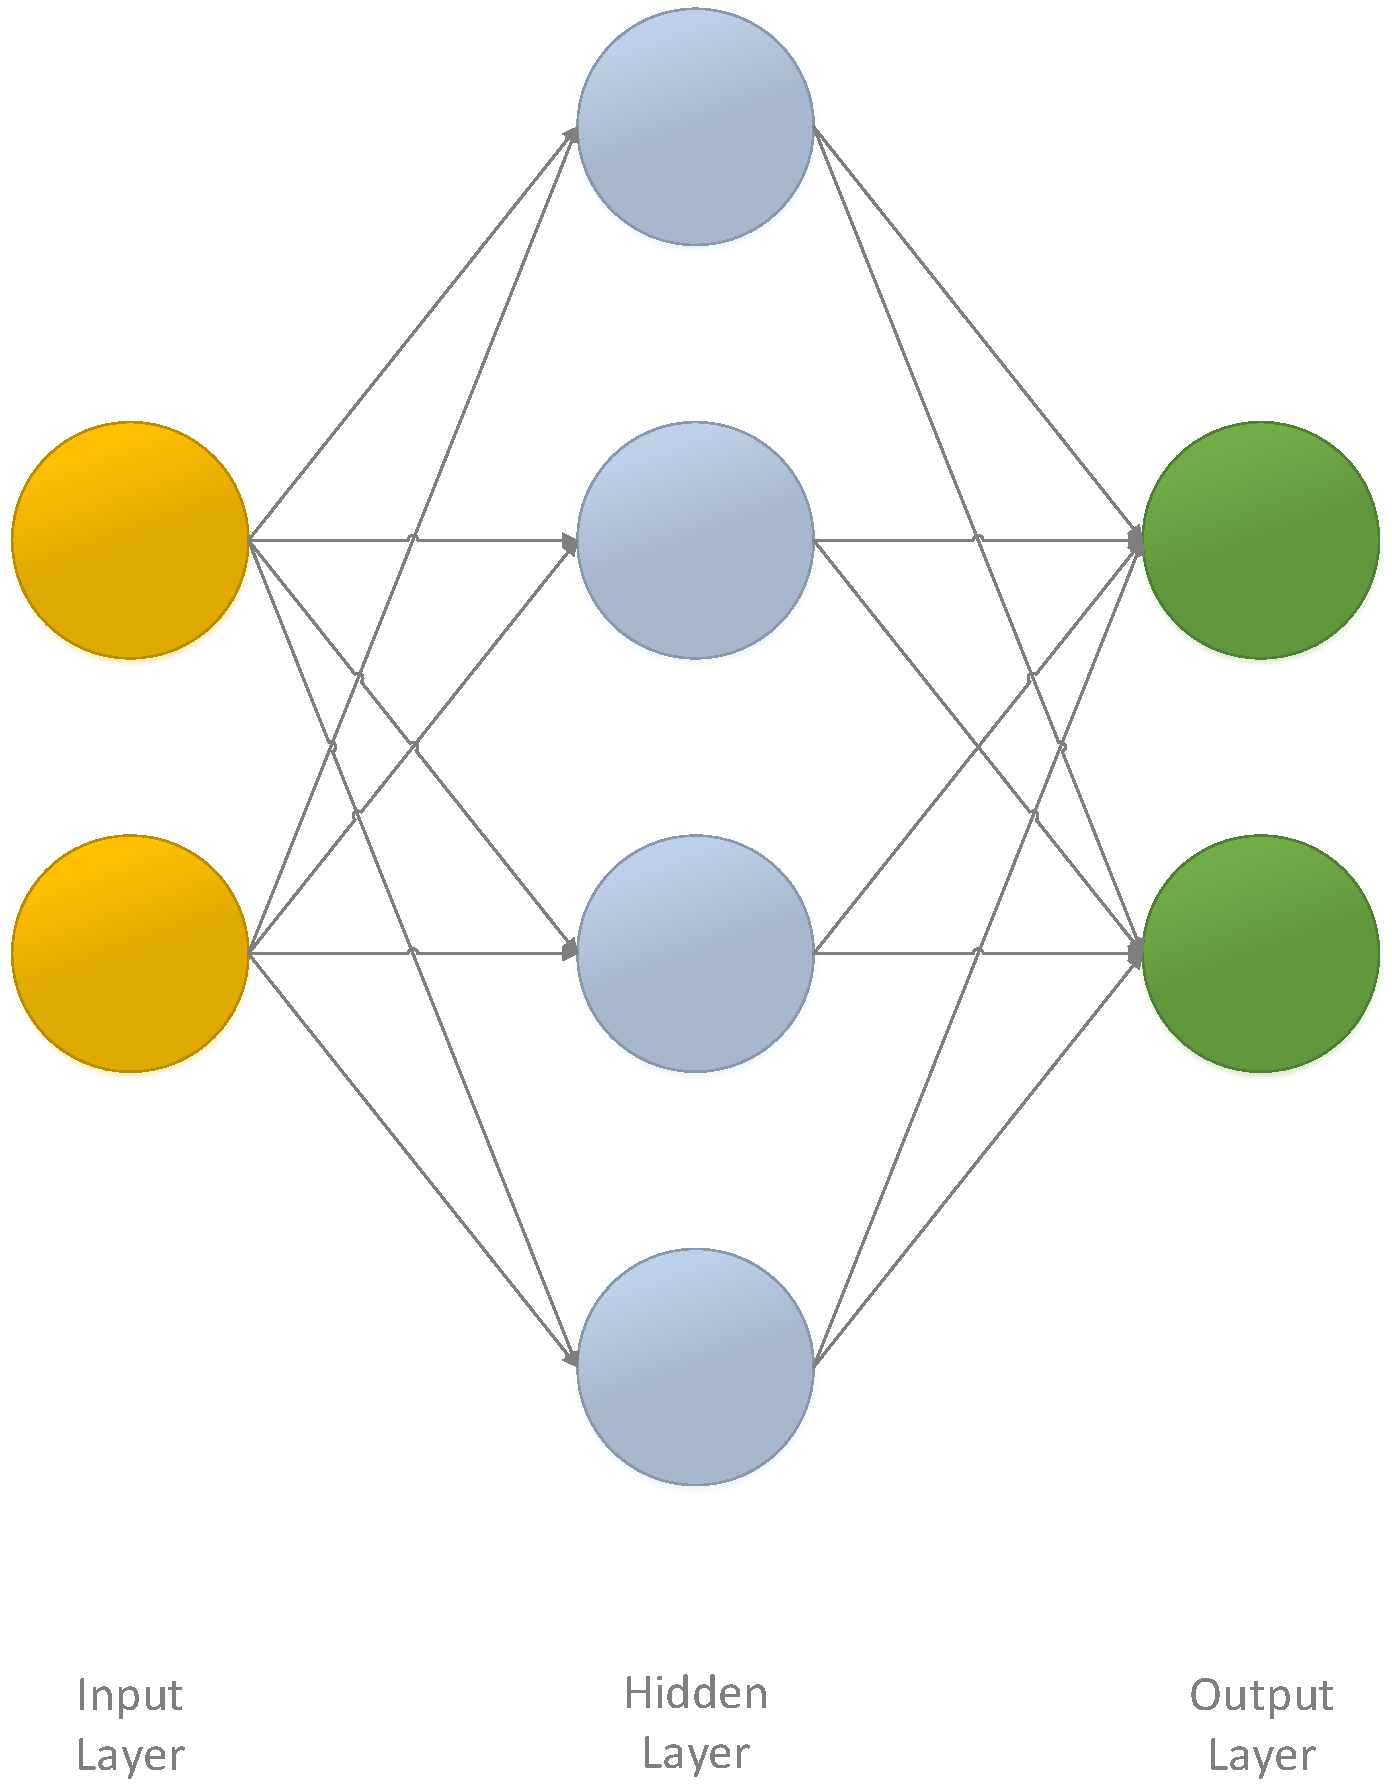
\includegraphics[width=\textwidth]{img/ann_1h}
		\caption{\glsentrylong{hl1}.}
		\label{fig:ann_1h}
	\end{minipage}
	\hfill
	\begin{minipage}[b]{0.45\textwidth}
		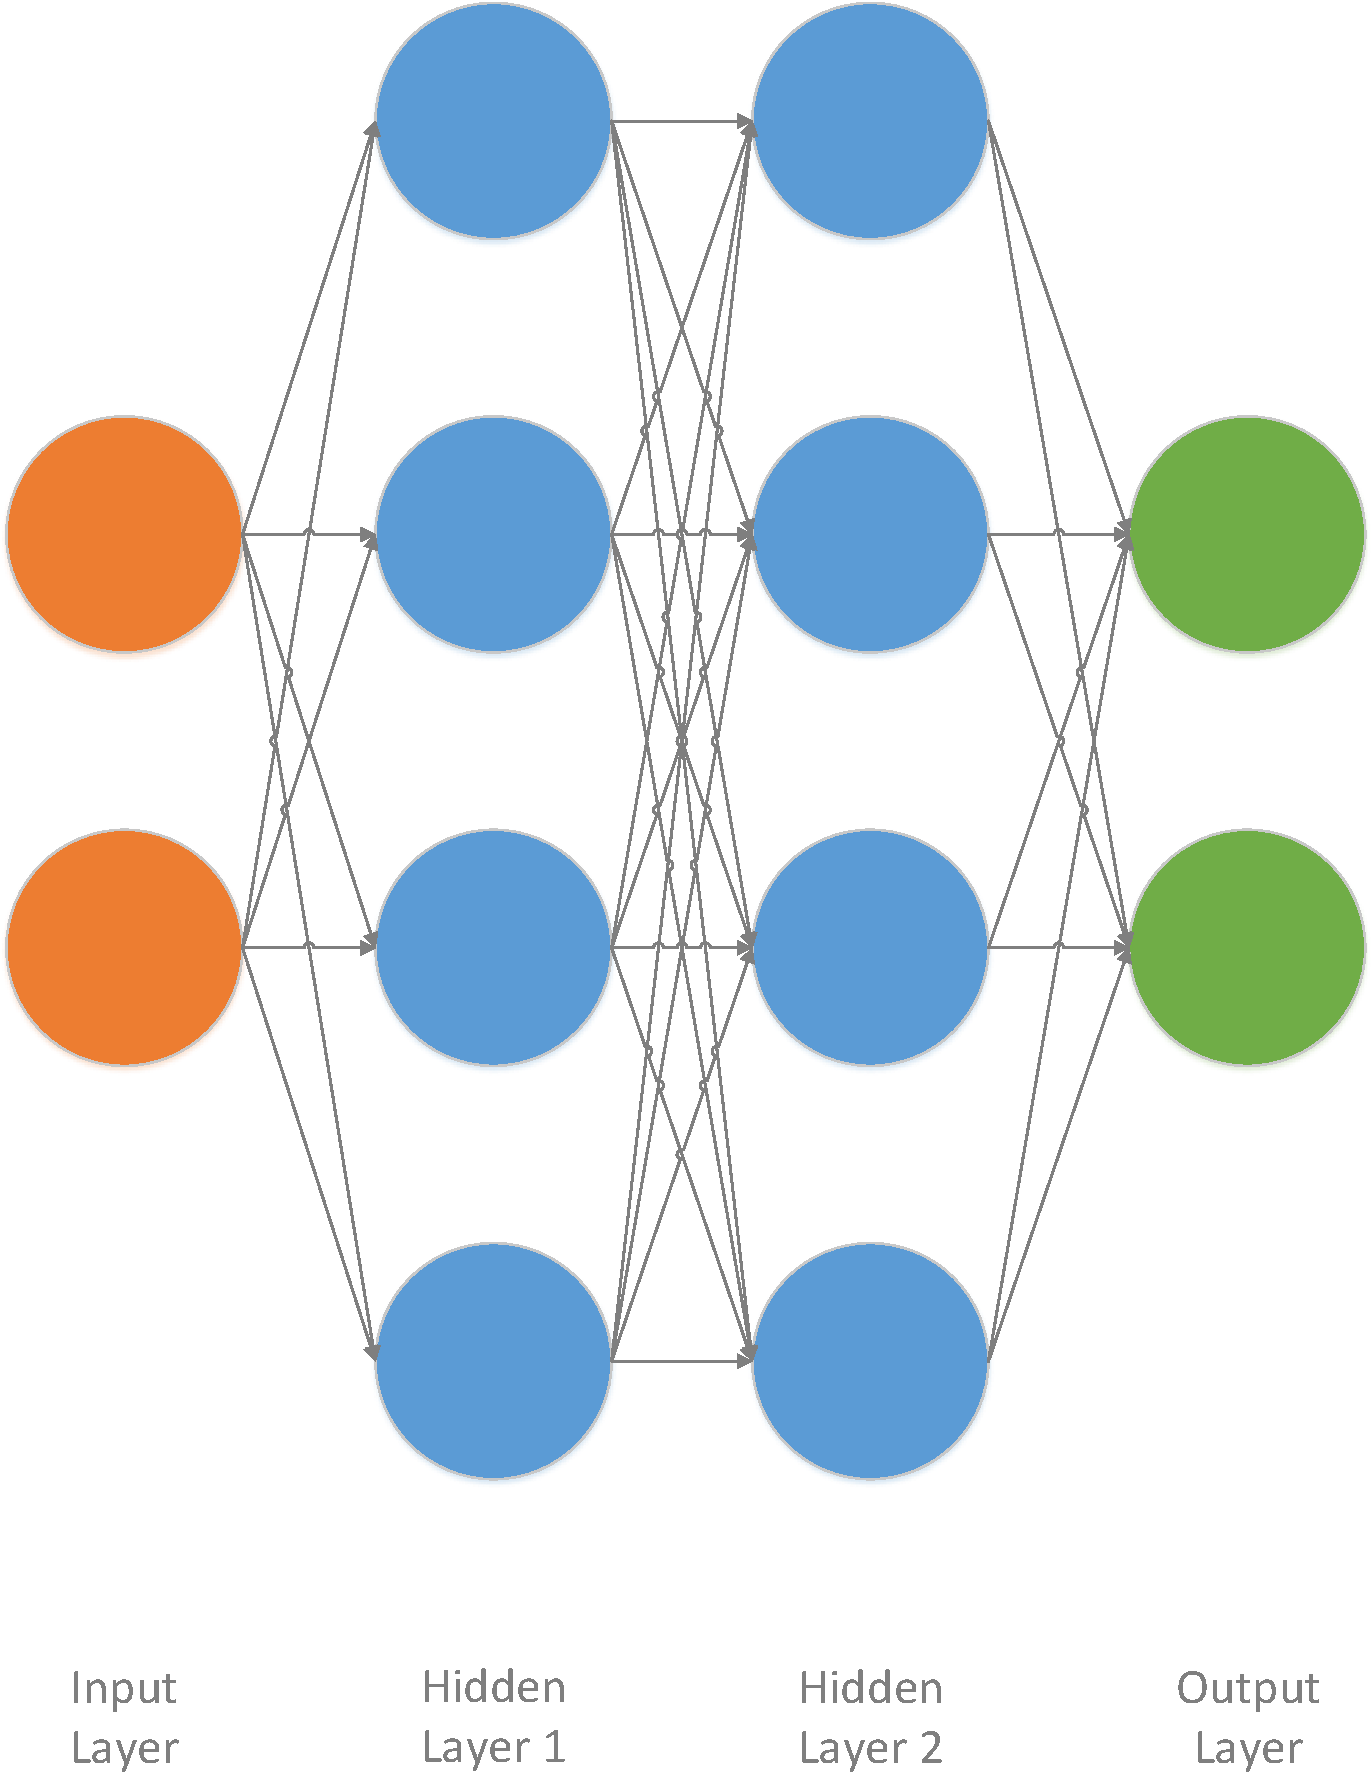
\includegraphics[width=\textwidth]{img/ann_2h}
		\caption{\glsentrylong{hl2}.}
		\label{fig:ann_2h}
	\end{minipage}
\end{figure}

Despite appearing more complex, \glspl{ann} rely on a similar approach for learning \ie updating their internal parameters, or in this case the whole network's synaptic connections, based on the \gls{sgd} method outlined in \subsecref{subsec:onpol_pred} \citep[p. 217]{Sutton2017}. This algorithm is called backpropagation and consists of doing a forward pass in which the activation function of each neuron is computed and then a backward pass computes the partial derivatives for each synaptic connection \citep[p. 218]{Sutton2017}.

As any other function approximation method, overfitting can be a problem for \glspl{ann} as well and it is particularly present for deep \glspl{ann} \citep[p. 218]{Sutton2017}. There are different techniques that can be used in order to mitigate this effect, with the most prominent one being the dropout method outlined by \citet{Srivastava2014}.

\subsection{\glsentrylong{onp} Control with Approximation}
\label{subsec:onpol_control}

Moving towards control with \gls{vfa}, we now focus on the approximation of the \gls{av} function $\hat{q} (s,a,\theta) \approx q_* (s,a)$ \citep[p. 229]{Sutton2017}.

For the special case of the so called one-step \gls{sarsa} method, its \gls{sgd} update for the \gls{av} function is defined as follows:

\begin{equation}
	\theta_{t+1} \doteq \theta_t + \alpha [ R_{t+1} + \gamma \hat{q} (S_{t+1}, A_{t+1}, \theta_t) - \hat{q} (S_t, A_t, \theta_t) ] \nabla \hat{q} (S_t, A_t, \theta_t)
\end{equation}

and this method has excellent convergence properties towards optimality \citep[p. 230]{Sutton2017}.

\subsection{\glsentrylong{op} Methods with Approximation}
\label{subsec:offpol_methods}

When moving towards the field of \gls{op} learning, one of the biggest problems that one might incur in is the convergence problem: \gls{op} learning with approximation is considerably harder compared to its tabular counterpart \citep[p. 243]{Sutton2017}. \gls{op} learning defines two policies, $\pi$ and $\mu$, where the former is the value function we seek to learn based on the latter \citep[p. 243]{Sutton2017}.

A new aspect being introduced in \gls{op} learning is the importance sampling concept, formally defined as follow:

\begin{equation}
\label{eq:importance_sampling}
	\rho_t \doteq \frac{\pi(A_t|S_t)}{\mu(A_t|S_t)}
\end{equation}

which can be used to ``warp the update distribution back to the \gls{onp} distribution, so that semi-gradient methods are guaranteed to converge.'' \citep[p. 243]{Sutton2017}.

During \gls{op} learning $\pi$ is defined as full greedy and $\mu$ is somewhat more exploratory \gls{ep} \citep[p. 243]{Sutton2017}.

For the purpose of this thesis, the focus has been put upon the episodic \gls{av} update algorithm, defined as follows:

\begin{equation}
	\theta_{t+1} \doteq \theta_t + \alpha \delta_t \nabla \hat{q} (S_t,A_t,\theta_t)\\
\end{equation}

where $\delta_t$ is defined as:

\begin{equation}
	\delta_t \doteq R_{t+1} + \gamma \overbrace{\sum_a \pi (a|S_{t+1}) \hat{q} (S_{t+1},a,\theta_t)}^{\max_a \hat{q} (S_{t+1},a,\theta_t)} - \hat{q} (S_t,A_t,\theta_t)
\end{equation}

what is to note here, is that the episodic \gls{op} algorithm does not use importance sampling as defined by \equref{eq:importance_sampling} \citep[p. 244]{Sutton2017}. \citet[p. 244]{Sutton2017} state that this approach is clear for tabular methods but it is rather a ``judgment call'' for methods using approximation functions and deeper understanding of the theory of function approximation is needed.

\subsection{\glsentrylong{pg} Methods}
\label{subsec:polgrad_methods}

Up until now all methods were based on the concept of learning values of actions and subsequently choosing the correct actions based on estimates, however, we now move our focus towards methods that actually learn a parametrized policy without needing value functions at all\footnote{\gls{ac} methods are an exception, where a learned value function is used in combination with \gls{pg} as a baseline in order to lower variance \citep{Sutton2017}.}  \citep[p. 265]{Sutton2017}. Parametrized policies work with probabilities that a specific action $a$ will be chosen at time $t$ if the agent finds itself in state $s$ at time $t$ with a weight vector $\theta$ \citep[p. 265]{Sutton2017}. For \gls{pg} methods it is crucial to learn the weight vector based on a performance measure $\eta(\theta)$ by trying to maximize and thus approximating the \gls{sga} of $\eta$ as follows:

\begin{equation}
	\theta_{t+1} \doteq \theta_t + \alpha \widehat{\nabla \eta (\theta_t)}
\end{equation}

where $ \widehat{\nabla \eta (\theta_t)}$ is nothing else than a stochastic estimate that approximates the gradient of $\eta(\theta)$ \citep[p. 265]{Sutton2017}.

For discrete action spaces, a suitable solution consists in forming parametrized numerical preferences $h(s,a,\theta) \in \mathbb{R}$ \citep[p. 266]{Sutton2017}. This means that the best action is given the highest probability according to a softmax distribution:

\begin{equation}
\label{eq:probabilistic_preferences}
	\pi(a|s,\theta) \doteq \frac{e^{h(s,a,\theta)}}{\sum_b e^{h(s,b,\theta)}}
\end{equation}

where $e \approx 2.71828$ \citep[p. 266]{Sutton2017}. Moreover, the preferences can be, as previously mentioned:

\begin{equation}
\label{eq:dot_preferences}
	h(s,a,\theta) \doteq \theta^\top \phi (s,a)
\end{equation}

simply linear in features \citep[p. 266]{Sutton2017}.

With these definitions in mind, one can formally define one of the very first \gls{mc} based \gls{pg} methods: \texttt{REINFORCE} \citep{Williams1992}. \citet{Williams1992} defines his \texttt{REINFORCE} algorithm by the following update function:

\begin{equation}
	\theta_{t+1} \doteq \theta_t + \alpha \gamma^t G_t \frac{\nabla_\theta \pi(A_t|S_t,\theta)}{\pi(A_t|S_t,\theta)}
\end{equation}

note that the vector $\frac{\nabla_\theta \pi(A_t|S_t,\theta)}{\pi(A_t|S_t,\theta)}$ is called eligibility vector and it is usually written in a more compact form of $\nabla \log \pi(A_t|S_t,\theta)$ by relying on the mathematical identity $\nabla \log x = \frac{\nabla x}{x}$ \citep[p. 271]{Sutton2017}. For the \texttt{REINFORCE} algorithm, its eligibility vector is defined as follows:

\begin{equation}
	\nabla_\theta \log \pi (a|s,\theta) = \phi (s,a) - \sum_b \pi (b|s,\theta) \phi (s,b)
\end{equation}

and this method has solid convergence properties \citep[p. 271]{Sutton2017}.

\subsubsection{\glsentrylong{pg} with Baseline}

\texttt{REINFORCE}, however, being a method based on \gls{mc} it might exhibit high variance and prove relatively slow in its learning rate \citep[p. 271]{Sutton2017}. By introducing a baseline $b(s)$ to compare the \gls{av}:

\begin{equation}
	\theta_{t+1} \doteq \theta_t + \alpha (G_t - \overbrace{b(S_t)}^{\text{Baseline}}) \frac{\nabla_\theta \pi(A_t|S_t,\theta)}{\pi(A_t|S_t,\theta)}
\end{equation}

one can achieve a positive effect towards diminishing variance of the update rule \citep[p. 271]{Sutton2017}.

\subsubsection{\glsentrylong{ac} \glsentrylong{pg}}

By introducing a base line, we have seen that variance can be lowered, however, the \texttt{REINFORCE} algorithm with a baseline is not a proper \gls{ac} method as its \gls{sv} function is only used as baseline and not as a critic \ie it is not used for bootstrapping \citep[p. 273]{Sutton2017}. By introducing bootstrapping we introduce bias and dependence of the quality of the approximated function, which in turn help to reduce variance and learn faster \citep[p. 273]{Sutton2017}. 

The only negative aspect still remaining is that \gls{pg} methods are still based on a full \gls{mc} update trajectory: this can be also mitigated by replacing the update function by \gls{td} learning approaches, such as those defined in \subsecref{subsec:td_learning} \citep[p. 273]{Sutton2017}. The formal definition of a one-step \gls{ac} update method is depicted as follows:

\begin{equation}
	\theta_{t+1} \doteq \theta_t + \alpha(R_{t+1} + \overbrace{\gamma \hat{v}(S_{t+1},w)-\hat{v}(S_t,w)}^{\text{\glsentryshort{td} update}}) \frac{\nabla_\theta \pi(A_t|S_t,\theta)}{\pi(A_t|S_t,\theta)}
\end{equation}

and this is now a fully online implementation that executes updates after each newly visited state \citep[p. 274]{Sutton2017}. 

\section{\glsentrylong{rl} Policies}
\label{sec:rl_policies}

Analog to \secref{sec:opt_policies}, the same policies are considered but now the \gls{rl} methods and techniques outlined in \secref{sec:rl_theory} are used to solve role resolution.

Different subsections are used in order to separate better the different approaches used for each type of policy:
\begin{enumerate*}
	\item Batch policy methods
	\item \gls{llqp} policy methods
	\item Other policy methods that do not fit in any of the previous categories.
\end{enumerate*}

The three key concepts required in order to effectively apply \gls{rl} techniques for role resolution in \glspl{wfms} are:
\begin{enumerate*}
	\item Correctly defined states and actions spaces
	\item Precise rewards definition
	\item Effective update method for the policy's internal parameters. 
\end{enumerate*}

\subsection{Prediction and Control Methods}

As previously outlined in \subsecref{subsec:onpol_pred}, \subsecref{subsec:onpol_control}, \subsecref{subsec:offpol_methods} and \subsecref{subsec:polgrad_methods} there are different prediction and control methods that can be applied.

\subsubsection{\glsentrylong{vfa}}

As mentioned in \secref{sec:rl_policies}, it is crucial to correctly define the states and actions space for each problem. Each request that the policy receives generates a policy job which is then passed in the internal evaluate method of the policy. Inside this method, for each policy job the state space $S$ is defined as a $m \times n+1$ matrix which contains all busy times of the potential candidates (\ie users) concatenated to the user's current service time for the job. Formally the state space is defined as depicted in \equref{eq:kbatch_sp}:

\begin{equation}
\label{eq:kbatch_sp}
	S_{m,n+1} = 
	\begin{bmatrix}
	a_1 & \cdots & a_1 \\
	a_2 & \cdots & a_2 \\
	\vdots & \ddots & \vdots \\
	p_{1,j} & \cdots & p_{i,j} \\
	\end{bmatrix}
\end{equation}

Since the possible actions are represented by the number of users, the state space is modeled such that for each possible actions a 1-D vector containing all busy times plus the service time of the user are present.

During the evaluation phase of a job the policy has to choose an action \ie a user, by taking into account the current state space and its internal $\theta$ parameters. By using a \gls{svfa} as defined in \equref{eq:function_approximation_dot}, the policy evaluates the highest score for each possible user.

As an example, let us consider a snippet of how a K-Batch policy using a linear \gls{svfa} performs its choices during its greedy phase: it iterates over all possible actions and performs the dot product between the state space and the corresponding $\theta$ vector and then maximizes the returned $Q$ value. This approach can be seen in \lstref{lst:e_greedy} and its respective \gls{svfa} in \lstref{lst:value_f_approx}.

\begin{lstlisting}[caption={\glsentrylong{ep} approach where if the policy is defined as greedy, actions are chosen by maximing the $Q$ values otherwise, with probability $\epsilon$ actions are randomly sampled.},label=lst:e_greedy,style=CustomPython]
if self.greedy:
    action = max(range(self.number_of_users), key=lambda action: self.q(state_space, action))
else:
    rnd = self.EPSILON_GREEDY_RANDOM_STATE.rand()
    if rnd < self.epsilon:
        action = self.EPSILON_GREEDY_RANDOM_STATE.randint(0, self.number_of_users)
    else:
        action = max(range(self.number_of_users), key=lambda action: self.q(state_space, action))
\end{lstlisting}

\begin{lstlisting}[caption=\glsentryshort{svfa} which performs the dot product between features $\phi$ and weight parameters $\theta$.,label=lst:value_f_approx,style=CustomPython]
def q(self, states, action):
    features = self.features(states, action)
    q = np.dot(features[action], self.theta[action])
    return q
\end{lstlisting}
 
 $Q$ values are however only one part of the requirements set by \gls{rl} methods, the next crucial aspect is defining the reward function. Since \gls{rl} agents are able to back-propagate what they have learned from one episode and thus update their internal factors, correctly defining a reward is a must. Since the goal for our domain is minimizing the maximum flowtime (from now on this metric will be referred to as lateness) of a job, the reward itself corresponds to the lateness of a job during a specific task. This can be evaluated a priori since for each policy job we know its internal parameters required to calculate the lateness \ie busy time of user $i$ plus the service time of user $i$ for job $j$, or formally $a_i+p_{ij}$.

 The last definition required in order to effectively apply the update on the policy's internal parameters $\theta$ is defining the \gls{sgd} method as outlined by \equref{eq:sgd_linear}. This method will give us the direction in which we have to update our internal $\theta$ parameters during our chosen update method and it is nothing more than the features themselves. As an example, refer to \lstref{lst:features_definition} for the concrete implementation.

\begin{lstlisting}[caption=Features definition which initializes a null matrix and fills the column corresponding to the chosen action by the policy.,label=lst:features_definition,style=CustomPython]
def features(self, states, action):
    features = np.zeros((self.number_of_users, self.number_of_users + 1))
    features[action] = states[action]
    return features
\end{lstlisting}

The features method outputs a matrix which has its values populated only for the actual chosen action. Let us assume our policy has chosen user 1 out of two possible users, then the state space looks as defined by \equref{eq:kbatch_sp_ex}:

\begin{equation}
\label{eq:kbatch_sp_ex}
	S_{2,3} = 
	\begin{bmatrix}
	a_1 & a_1 \\
	a_2 & a_2 \\
	p_{1,j} & p_{2,j} \\
	\end{bmatrix}
\end{equation}

and its features vector looks as defined by \equref{eq:kbatch_features_ex}:

\begin{equation}
\label{eq:kbatch_features_ex}
	\phi_{2,3} = 
	\begin{bmatrix}
	a_1 & 0 \\
	a_2 & 0 \\
	p_{1,j} & 0 \\
	\end{bmatrix}
\end{equation}

\subsubsection{\glsentrylong{pg}}

With \gls{pg} methods the approach on how an action is chosen is shifted. Instead of maximizing a $Q$ value through internal $\theta$ parameters in order to choose the ``best greedy'' action, we now have probabilistic choices. As already outlined in \subsecref{subsec:polgrad_methods}, having a probabilistic policy $\pi$ means that the best action is now chosen according to the highest probability which follows a softmax distribution as defined in \equref{eq:probabilistic_preferences} and its implementation can be seen in \lstref{lst:softmax_probabilities}.

\begin{lstlisting}[caption=Softmax distribution of preferences probabilities.,label=lst:softmax_probabilities,style=CustomPython]
def policy_probabilities(self, busy_times):
    probabilities = [None] * self.number_of_users
    for action in range(self.number_of_users):
        probabilities[action] = np.exp(np.dot(self.features(busy_times, action), self.theta)) / sum(np.exp(np.dot(self.features(busy_times, a), self.theta)) for a in range(self.number_of_users))
    return probabilities
\end{lstlisting}

The policy probabilities method takes as input parameter the current state space and computes for each user its probability according to the current internal $\theta$ parameter as defined in \equref{eq:dot_preferences}. The result of this method is a 1-D probabilities vector corresponding to a preference to assign a job to a specific user, where the index of the vector corresponds to the user and the value to its preference. Based on this preferences vector, the policy then computes a weighted random choice among all users, as can be seen in \lstref{lst:prob_user_choice}.

\begin{lstlisting}[caption=Probabilistic user choice by accounting for preferences weights.,label=lst:prob_user_choice,style=CustomPython]
chosen_action = self.RANDOM_STATE_PROBABILITIES.choice(self.number_of_users, p=probabilities)
\end{lstlisting}

\subsubsection{\glsentrylongpl{ann} as Function Approximation}

Up to this point we have used linear functions for the approximation of the $Q$ value for the different policies. As mentioned in \subsecref{subsec:onpol_pred}, \glspl{ann} can be used for nonlinear function approximation. The assignment problem  poses itself very well for this kind of application, in which we model our input layer as a 1-D vector containing all required information such as waiting time $w$ of job $j$, service time $p_{ij}$ of user $i$ for job $j$ and busy time $a_i$ of user $i$. By following a \gls{pg} approach, we can categorize the output layer of our \glspl{ann} using a softmax categorization function, mapping the preferences of job $j$ to user $i$ assignment as probabilities. \lstref{lst:ann_1h} show the modeling of a single layer perceptron in \gls{tf}: one hidden layer connects the state space \ie input to the \glspl{ann}, together with its weights and biases, creates an activation function and maps the prediction layer \ie output, with a softmax classification.

\begin{lstlisting}[caption={Modeling of a single perceptron in \glsentryshort{tf}, where the initial hidden layer is composed as the product between the input layer and its corresponding weights plus the corresponding biases by using an \glsentryshort{elu} activation function.},label=lst:ann_1h,style=CustomPython]
with tf.name_scope("neural_network"):
	layer_1 = tf.add(tf.matmul(state_space_input, weights['h1']), biases['b1'])
	layer_1 = tf.nn.elu(layer_1)
	pred = [tf.add(tf.matmul(layer_1, weights['out'][b]), biases['out'][b]) for b in range(batch_input)]
	probabilities = [tf.nn.softmax(pred[b]) for b in range(batch_input)]
\end{lstlisting}

In order to update the \glspl{ann}, a backpropagation has to take place. Such an update can both be made following a \gls{mc} or \gls{td} approach (refer to \subsecref{subsec:update_methods} for a detailed distinction between these two update methods). As outlined in \subsecref{subsec:onpol_pred}, we follow a \gls{sgd} approach in which we update all the synaptic connections by computing the partial derivatives of all the weights. \lstref{lst:mc_backpropagation} shows how the backpropagation for an \glspl{ann} following a \gls{mc} update method is done.

\begin{lstlisting}[caption={Backpropagation algorithm following a \glsentryshort{mc} update approach. Initially rewards are discounted which are eventually used to calculate the multiplying factor for the partial derivatives.},label=lst:mc_backpropagation,style=CustomPython]
def train(self):
    for t, (state, output, choices) in enumerate(self.history):
        disc_rewards = self.discount_rewards(t)
        tmp_choices = [choice for choice in choices if choice is not None]
        for job_index, chosen_user in enumerate(tmp_choices):
            prob_value = output[job_index].flatten()[chosen_user]
            reward = disc_rewards[job_index]
            factor = reward / prob_value
            grad_input = np.zeros((self.number_of_users, 1))
            grad_input[chosen_user] = 1.0
            self.sess.run(self.apply[job_index], {self.state_space_input: state, self.gradient_input: grad_input, self.factor_input: factor})
\end{lstlisting}

\subsection{Update Methods}
\label{subsec:update_methods}

As outlined in \subsecref{subsec:mc} and \subsecref{subsec:td_learning}, there are mainly two different methods to update the policy's internal $\theta$ parameters \ie \gls{mc} and \gls{td}. Let us take the example outlined by \citet[p. 130]{Sutton2017} of leaving the office and getting home and the respective updates proposed by the two update methods. \figref{fig:mc_td} shows the graphical updates proposed by the two update methods.

\fig[\textwidth]{mc_td}{\glsentryshort{mc} and \glsentryshort{td} proposed updates comparison. \glsentryshort{mc} approaches have to wait until the end of an episode in order to update since they require a full episode to effectively discount rewards, compared to \glsentryshort{td} approaches that are able to update at each following time step $t+1$. Adapted from \citet[p. 130]{Sutton2017}.}{fig:mc_td}

As it can be clearly seen, the main deference lays in when the actual updating takes place. On one hand, the \gls{mc} method needs to reach the end of an entire episode \eg here it consists of actually arriving home, in order to fully back-propagate its learned value and update the $\theta$ parameters. On the other hand, \gls{td} is much more flexible and robust since it executes its updates at each time step, hence its name: \gls{td}.

For a formal overview of the difference between the two update methods, refer to \equref{eq:mc_update} for the \gls{mc} update and to \equref{eq:td_update} for the \gls{td} update.

For the case at hand, this means that training the policies has to be done in a different fashion for the two update methods: while \gls{td} based policies can be updated ``on-the-fly'', \gls{mc} methods require batch training sessions \ie episodes, at the end of which they can effectively learn and update their internal $\theta$ parameters to be used for the next episode. Not only the training approach is different, but the logic of the policy itself is also different: for \gls{td} based policies, the update method is being called internally since the policy knows its temporal steps, while for \gls{mc} based policies the policy itself cannot know a priori when an episode will finish and thus must relay on an ``artificial'' definition of such. The overall overhead is also different since \gls{mc} based policies have to keep track of their whole episode history which usually is composed of the state space, chosen action and reward at time step $t$.

\citet{Sutton2017} outline a qualitative comparison between both update methods which can be found summarized in table \tabref{tab:mc_td_comp}.

% Please add the following required packages to your document preamble:
% \usepackage{booktabs}
\begin{table}[!ht]
	\centering
		\begin{tabular}{@{}lll@{}}
		\toprule
		Characteristic & \glsentryshort{mc}                     & \glsentryshort{td}                               \\ \midrule
		Bootstrap      & No                     & Yes                              \\
		Update Time    & End of episode         & Each time step                   \\
		Discount       & Required               & Not required                     \\
		Convergance    & Good                   & Very Good                        \\
		Learning Rate  & Slow for long episodes & Very fast even for long episodes \\ \bottomrule
		\end{tabular}
	\caption{Qualitative comparison between \glsentryshort{mc} and \glsentryshort{td} update methods. Adapted from \citep[p. 130]{Sutton2017}.}
	\label{tab:mc_td_comp}
\end{table}

\subsection{Batch Size Emulation}
\label{subsec:batch_size_emulation}

Correctly defined state spaces is a crucial requirement for effective \gls{rl} methods. \gls{llqp} policies are relatively easy to be modeled, on the other hand policies with batch sizes require a more meticulous consideration. By introducing a batch size that retains jobs in its global queue \ie all batch sizes $K>1$, not only the role resolution plays a role, but the ordering of the assignment influences greatly the final outcome as well. Let us consider a simple case with number of jobs $m=3$, number of users $n=2$ and at time step $t$. \tabref{tab:users_service_times_example} summarizes the service times $p_{ij}$ in time units $t$ of both users for all three jobs.

% Please add the following required packages to your document preamble:
% \usepackage{booktabs}
\begin{table}[!ht]
	\centering
		\begin{tabular}{@{}llll@{}}
		\toprule
		User   & Job 1 & Job 2 & Job 3 \\ \midrule
		User 1 & $1$     & $2$     & $3$     \\
		User 2 & $4$     & $5$     & $6$     \\ \bottomrule
		\end{tabular}
	\caption{Sample service times of both users for all three jobs.}
	\label{tab:users_service_times_example}
\end{table}

It is clear that the ordering of the jobs assigned has an impact on the final outcome. \figref{fig:user_job_assignment_order} outlines a possible conformation where user 1 receives job 1 while user 2 gets assigned to jobs 2 and 3 respectively. In this case, job 1 is started at $t$ and is finished at $t+1$, job 2 is started at $t$ and is finished at $t+5$ and job 3 is started at $t+5$ and is finished at $t+11$. The respective lateness per job is: $1$ for job 1, $5$ for job 2 and $6$ for job $3$.

By changing the assignment order (refer to \figref{fig:user_job_assignment_order2} for a graphical representation), the final outcome changes as well: In this case, job 1 is started at $t+2$ and is finished at $t+3$, job 2 is started at $t$ and is finished at $t+2$ and job 3 is started at $t$ and is finished at $t+6$. The respective lateness per job is: $1$ for job 1, $2$ for job 2 and $6$ for job $3$. By merely changing the assignment order a $2.5$ speedup factor in lateness is observed for job 2.

\begin{figure}[!ht]
	\centering
	\begin{minipage}[b]{0.45\textwidth}
		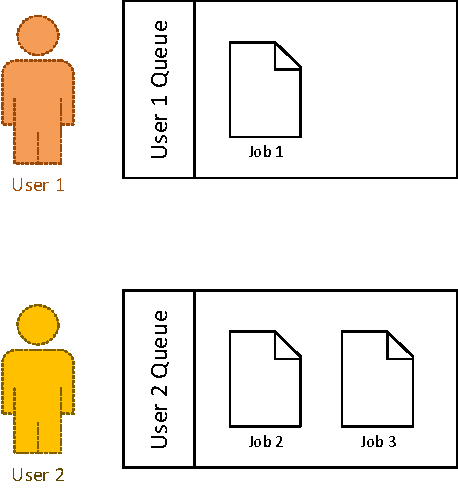
\includegraphics[width=\textwidth]{img/user_job_assignment_order}
		\caption{User 1 receives job 1 while user 2 receives jobs 2 and 3.}
		\label{fig:user_job_assignment_order}
	\end{minipage}
	\hfill
	\begin{minipage}[b]{0.45\textwidth}
		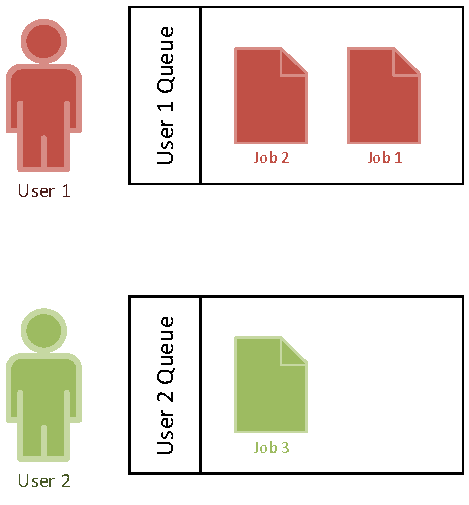
\includegraphics[width=\textwidth]{img/user_job_assignment_order2}
		\caption{User 1 receives jobs 2 and 1 while user 2 receives job 3.}
		\label{fig:user_job_assignment_order2}
	\end{minipage}
\end{figure}

\subsecref{subsec:rl_others} outlines three different types of policies (refer to \tabref{tab:rl_others_policies_overview} for a detailed explanation of the policies) that take into account the previously outlined job assignment ordering principle and exploit it in their state space modeling. This is done by means of integrating an additional parameter $B$ that defines how many jobs have to be considered when trying to optimally assign jobs queuing in the global queue to users. This is done by listing all possible combinations by accounting for the job order as well. Refer to \lstref{lst:wz_combinations} for the actual implementation.

\begin{lstlisting}[caption=State space modeling by considering $B$ jobs from the global queue and integrating all possible combinations.,label=lst:wz_combinations,style=CustomPython]
combinations = list(itertools.product(range(self.number_of_users), repeat=self.wait_size))
for i, combination in enumerate(combinations):
    state_space[i] = a + [p[user_index][job_index] for job_index, user_index in enumerate(combination)]
\end{lstlisting}

This approach effectively simulates batch policies with batch sizes $K>1$.